\begin{figure}[htbp]
\centering
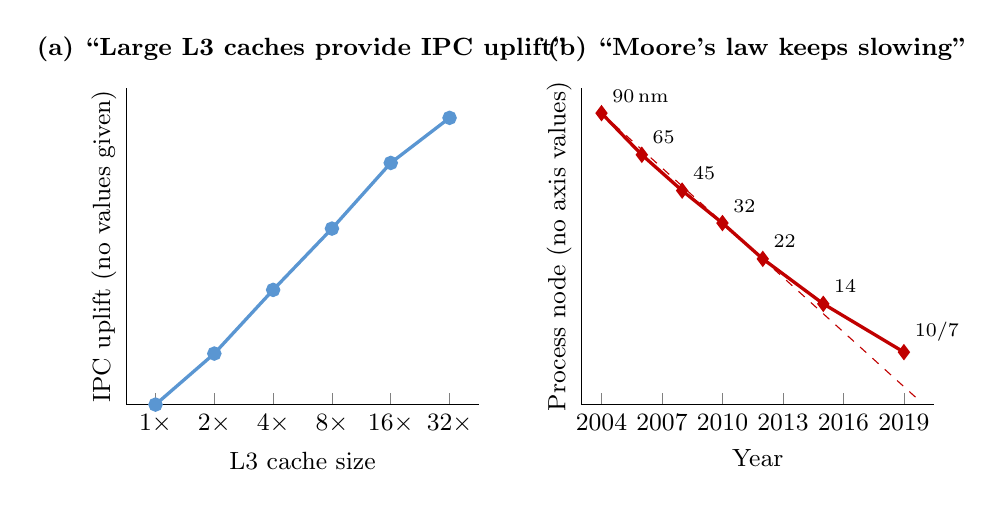
\begin{tikzpicture}
\begin{axis}[
  name=a, width=0.5\textwidth, height=5.6cm,
  title={\small\bfseries (a) ``Large L3 caches provide IPC uplift''},
  xmode=log, log basis x=2, xtick={1,2,4,8,16,32}, xticklabels={1$\times$,2$\times$,4$\times$,8$\times$,16$\times$,32$\times$},
  xticklabel style={font=\small}, xlabel={L3 cache size}, xlabel style={font=\small},
  ymin=0, ymax=8, ytick=\empty, ylabel={IPC uplift (no values given)}, ylabel style={font=\small},
  axis x line*=bottom, axis y line*=left]
\addplot[very thick, color={rgb,255:red,90;green,150;blue,210}, mark=*] coordinates {(1,0) (2,1.29) (4,2.90) (8,4.45) (16,6.11) (32,7.25)};
\end{axis}
\begin{axis}[
  at={(a.east)}, anchor=west, xshift=1.3cm, width=0.5\textwidth, height=5.6cm,
  title={\small\bfseries (b) ``Moore's law keeps slowing''},
  xmin=2003, xmax=2020.5, xtick={2004,2007,2010,2013,2016,2019}, xticklabel style={font=\small, /pgf/number format/1000 sep={}},
  xlabel={Year}, xlabel style={font=\small},
  ymin=-900, ymax=-520, ytick=\empty, ylabel={Process node (no axis values)}, ylabel style={font=\small},
  axis x line*=bottom, axis y line*=left, clip=false]
\addplot[very thick, color={rgb,255:red,192;green,0;blue,0}, mark=diamond*,
  nodes near coords, point meta=explicit symbolic, nodes near coords style={font=\scriptsize, color=black, anchor=south west}]
  coordinates {(2004,-550)[90\,nm] (2006,-600)[65] (2008,-643)[45] (2010,-682)[32] (2012,-725)[22] (2015,-779)[14] (2019,-837)[10/7]};
\addplot[thin, dashed, color={rgb,255:red,192;green,0;blue,0}, domain=2004:2019.6] {-550-21.9*(x-2004)};
\end{axis}
\end{tikzpicture}
\caption[Two of the charts with which AMD's ISSCC~2022 presentation opens, redrawn]{Two of the charts with which AMD's ISSCC~2022 presentation opens, redrawn \cite[slides~5--6]{wuu2022vcache}. (a)~IPC uplift against L3 size on a linear uplift axis. The slide gives no values and names no workloads, so only the shape is shown: each doubling of the L3 up to 16$\times$ adds a similar step, and the last doubling a smaller one. (b)~Process node against year of introduction, with the dashed line continuing the pace of 2004--2012. The slide gives no axis values, so only the positions are reproduced: after 22\,nm each node lies above the earlier trend, that is, it arrived later than that pace would predict. Positions are read from the slide and are approximate.}
\label{fig:isscc-charts}
\end{figure}
